\documentclass[tikz]{standalone}
\usepackage{tikz}
\usetikzlibrary{arrows.meta, positioning, shapes.geometric}

\begin{document}

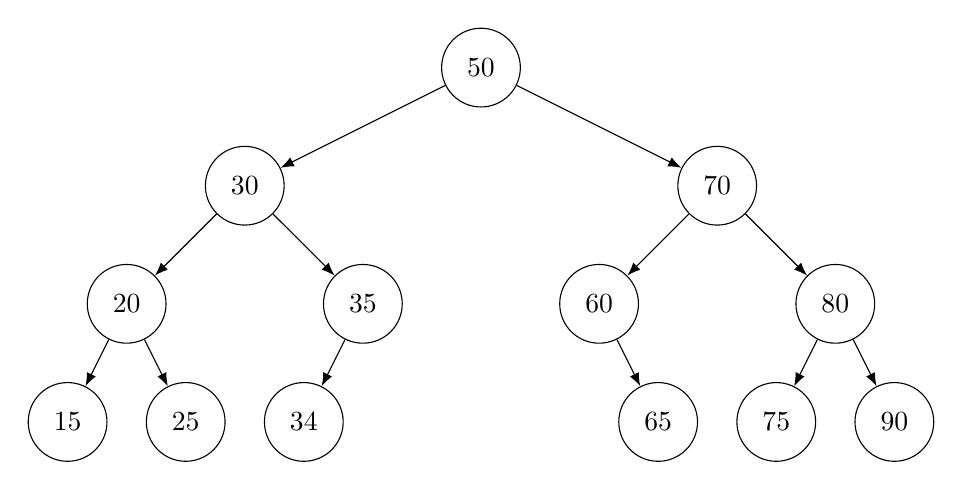
\begin{tikzpicture}[
    every node/.style={circle, draw, minimum size=1cm},
    level 1/.style={sibling distance=6cm},
    level 2/.style={sibling distance=3cm},
    level 3/.style={sibling distance=1.5cm},
    edge from parent/.style={draw, -Latex}
]

% Wurzelknoten
\node {50}
    child {node {30} 
        child {node {20}
            child {node {15}}
            child {node {25}}
        }
        child {node {35}
            child {node {34}}
            child[missing] {}
        }
    }
    child {node {70}
        child {node {60}
            child[missing] {}
            child {node {65}}
        }
        child {node {80}
            child {node {75}}
            child {node {90}}
        }
    };

\end{tikzpicture}

\end{document}
